\documentclass[12pt]{article}
\usepackage{fontspec}
\usepackage{amsmath, amssymb}
\usepackage{mathtools}
\usepackage{graphicx}
\usepackage{hyperref}
\usepackage{geometry}
\usepackage{float}
 \geometry{
 a4paper,
 total={170mm,257mm},
 left=20mm,
 top=20mm,
 }
\usepackage{fancyhdr}
\usepackage{titlesec}
\usepackage{siunitx}
\usepackage{caption}
\usepackage{polyglossia}
\usepackage{placeins}
\usepackage{tabularx}

\setmainfont{Calibri}
\setmainlanguage{greek}
\setotherlanguage{english}
\graphicspath{ {./figures/} }

\pagestyle{fancy}
 \setlength{\headheight}{14.5pt}
\fancyhf{}
\fancyhead[L]{Αριστοτέλειο Πανεπιστήμιο Θεσσαλονίκης}
\fancyhead[R]{Διπλωματική Εργασία}
\fancyfoot[C]{\thepage}
\fancyfoot[R]{}


% Title formatting
\titleformat{\section}{\normalfont\Large\bfseries}{\thesection}{1em}{}
\titleformat{\subsection}{\normalfont\large\bfseries}{\thesubsection}{1em}{}
\begin{document}
\begin{titlepage}
\newgeometry{margin=2cm, tmargin=3cm, bmargin=3cm}
\centering
\begin{figure}[H]
\centering

\includegraphics[width=0.8\textwidth]{banner-horizontal-black300ppi.png}\par % Image on top of title
\end{figure}
%\textcolor{black}{\large \bfseries Αριστοτέλειο Πανεπιστήμιο Θεσσαλονίκης\\}\par
\vspace{18pt}
\textcolor{black}{\Large \bfseries Τμήμα Ηλεκτρολόγων Μηχανικών\\και Μηχανικών Υπολογιστών\\}\par
\vspace{1cm}
\vfill
\textcolor{black}{\Large \bfseries Διπλωματική Εργασία}\par
\vspace{0.8cm}
\textcolor{black}{\Large \bfseries Δοκιμαστική Έκδοση}\par

\vspace{0.5cm} % Adjust vertical spacing here
\vfill
\newcolumntype{L}{>{\raggedright\arraybackslash}X}%
\newcolumntype{R}{>{\raggedleft\arraybackslash}X}%
{\large
\def\arraystretch{1.3}
\begin{tabularx}{\textwidth}{ R|L }
\textbf{Όνομα Φοιτητή}  & Βαπόρης Δημήτριος          \\
\textbf{ΑΕΜ}  & 10625 \\
\textbf{Επιβλέπων Καθηγητής} & Ντελόπουλος Αναστάσιος\\
\end{tabularx}
}
\vspace{0.5cm}
\vfill
\textcolor{black}{\large \bfseries Εαρινό Εξάμηνο 2026}\par
\end{titlepage}

\restoregeometry

\tableofcontents
\newpage
\section{Εισαγωγή}

\section{Proposed Method}

A combination of Contrastive Learning methods and a diffusion generation mechanism is proposed, known as a Latent Diffusion Model (LDM). The following schematics aim to provide a visual explanation of the process.

\subsection{Contrastive Learning}

\begin{figure}[h]
	\centering
	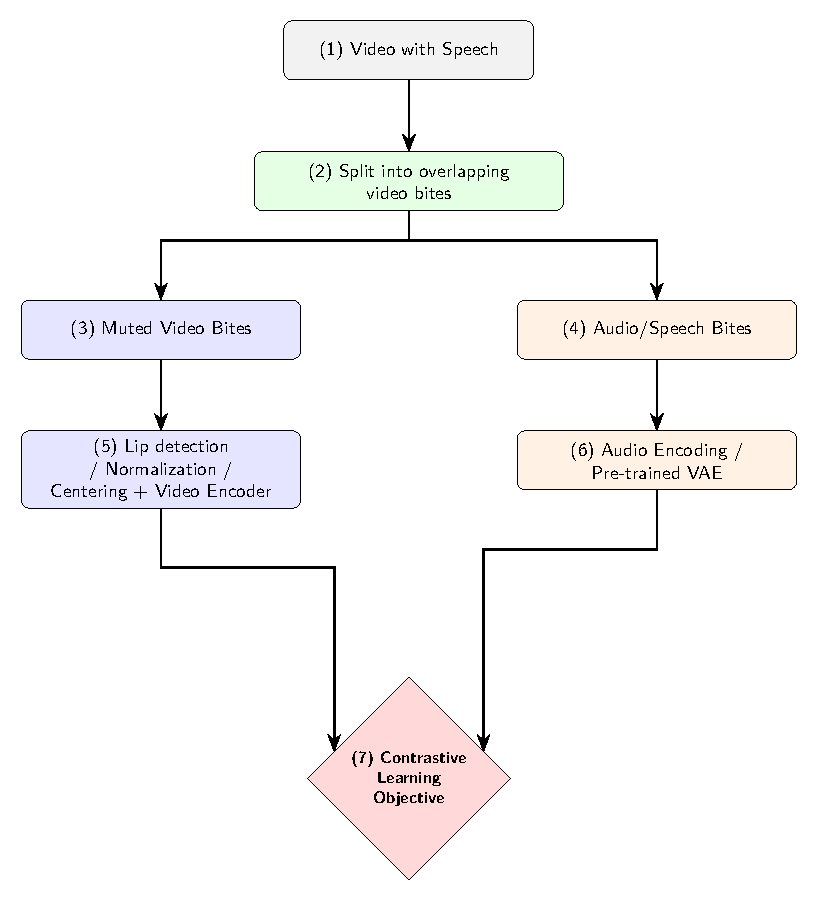
\includegraphics{Contrastive_Learning.pdf}
	\caption{The Contrastive Learning part of the proposed method}
\end{figure}

The method proposed is very similar to the one proposed in Diff-Foley \cite{Diff-Foley}. More specifically, each step of the above schematic is explained below:

(1): The process begins with data from a video with speech.

(2): The video is divided into overlapping video bites (overlap \% is a tunable parameter) of length capable of depicting a specific sound (syllable?) made during speech (around 0.1-0.3 seconds, also a tunable parameter).

(3), (4): The data is split into muted video bites and audio/speech bites.

(5): The data of the muted video bites is pre-processed using a combination of the following techniques:
\begin{itemize}
\item Face/Lip Detection: To avoid meaningless information connected to speech (i.e. background color, clothes of speaker...) a face/lip detection mechanism is used to reduce the size of data passed to next stages.
\item Normalization/Centering: Prevent the model from confusing head tilt/shake as an important part of speech (could be redundant based on architecture used later).
\item Possible conversion to Grayscale instead of RGB to further reduce the data incorporated.
\item Masking: Two forms of masking are possible, temporal and spatial. Temporal masking involves adding noise to (or completely covering) a relatively small number of frames of the video bite in their entirety, whereas spatial masking constitutes of adding noise to specific areas of the video bite (i.e. near the left part of the lip) for the entire video bite (or, again, covering/removing them entirely).
\end{itemize}
The final processed data is passed into the Video Encoder (i.e. VideoMAE \cite{VideoMAE}, works with a high masking percentage). Meta's VideoMAE v2 base model from Hugging Face was chosen \cite{VideoMAEv2}.

(6): The audio is also processed and encoded, using the Mel-spectogram. A Pre-trained Audio Variational Autoencoder (VAE) is used, since it is trained to both encode and decode to and from the resulting latent space, while retaining phase information (crucial for correct reconstruction and alignment of lip movements and sounds generated). Examples of architectures to be considered: HTS-AT \cite{HTS-AT} or the VAE used in AudioLDM \cite{AudioLDM}. Due to issues with the dependencies of the video encoder alongside the audio encoder, EnCodec from Meta was chosen \cite{EnCodec}.

(7): Lastly, the Contrastive Learning Objective is applied, by the result of which the fine-tuning of the encoders is driven. The Contrastive Learning Objective is very similar to the one presented in Diff-Foley \cite{Diff-Foley}, containing a Semantic Contrast and a Temporal Contrast. The Semantic Contrast aims to maximize the similarity score of video-audio bite pairs coming from the same video while minimizing the score of video-audio bite pairs coming from different ones (if not using many different videos with different speakers, then totally different parts of the video, maybe with a completely different context/emotion/tone of the speaker). The Temporal Contrast aims to maximize the similarity of video-audio bite pairs that come from the same time segment of the video, whereas it minimizes the similarity score of pairs coming from different time segments, making precise timing crucial (this is why an overlap is also proposed, to enhance learning of precise timing).

\subsection{Generation by Diffusion}

Having completed the training of the Contrastive Learning part, the outputs of the Video Encoder as well as the VAE are aligned in a common latent space, meaning that muted video bites are projected via the Video Encoder to a point in the latent space that resides close to the projection of the missing sound/speech, after being passed through the VAE. This fact is taken advantage of in order to drive or rather condition the diffusion generation process, which can be visualized below.

\begin{figure}[h]
	\centering
	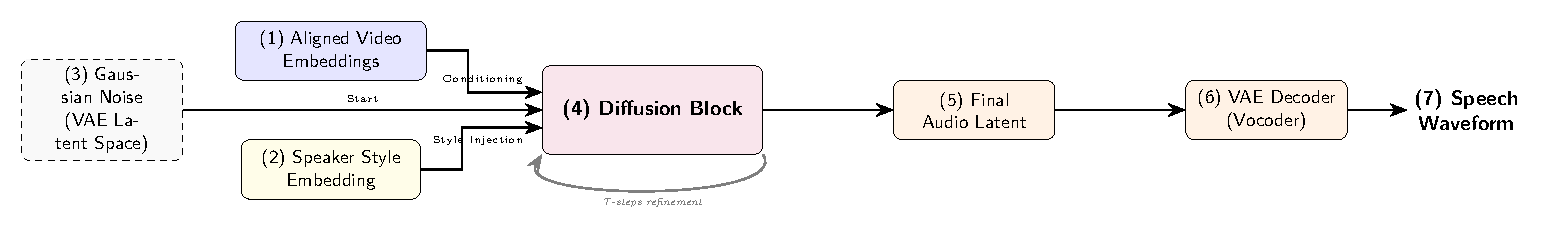
\includegraphics[width=\textwidth]{Generation.pdf}
	\caption{The Generation by Diffusion part of the proposed method}
\end{figure}

Below, a brief explanation of the modules above is included.

(1): As discussed previously, having completed the Contrastive Learning part of the method creates an aligned latent space, meaning that the embedding resulting from the video bite for which speech is being generated can be used as conditioning for the diffusion process (maybe also neighboring video bites?).

(2): An optional part of the process that may help alleviate robotic sound and generalize the process is the usage of the speaker's style embedding as a secondary conditioning mechanism (a ``style injection'') for the diffusion. Using pre-trained Speaker Encoders (like WavLM \cite{WavLM}) that encapsulate information like the speaker's tonality from a reference speech clip, the result of the diffusion process may be steered so as to attempt to ``match'' the desired speaker tone.

(3): The first step of the diffusion process described below is a Gaussian Noise vector in the latent space of the Audio VAE. The diffusion process aims to ``denoise'' the initial vector and finally create a vector in the latent space that may then be decoded as a speech segment valid for the video bite at hand, conditioned (driven) by the aligned video embeddings and, optionally, the speaker's style. Importantly, during sampling, a scaled version of noise is added in each step of the diffusion process except for the last one (the one that results in the outcome), as shown in DDPM \cite{DDPM}.

(4): The Diffusion Block is the cornerstone of generation for the proposed method. During training, the Diffusion Block receives an Audio Latent as well as the corresponding Video Latent created from the VAE and the Video Encoder respectively. Since the objective is speech generation, Gaussian Noise is added to the Audio Latent. The objective of the Diffusion Block during training is, given the noisy Audio Latent and the Video Embedding, to predict how much noise was added to the Audio Latent. The loss function stems from the error in the actual noise added versus the predicted noise. Having completed training, during inference (generation), random noise is sampled for the first step (as discussed in 3). The Video Embedding serves as a conditioning mechanism, driving the process towards a less noisy Audio Latent that, after enough steps (also a tunable parameter), resides close in the Aligned Latent Space to the Video Embedding (hopefully...). The optional Speaker Style Injection acts as a constant bias that ensures the resulting denoised latent maps to a speech segment with the same tonal characteristics of the target speaker. 

(5): After T steps of refinement in the inference process, a final Audio Latent is produced.

(6): This final Audio Latent is then passed into the VAE Decoder.

(7): The result of the VAE Decoder is now a speech waveform with length equal to the length of the initial video bite.

Following this process, a speech waveform is produced for every video bite of the desired video. However, simply adding these bites on top of one another to create the final speech segment would create discontinuities in the sound, especially at the end and the beginning of each bite. Thus, a need for combination of the speech waveforms is presented, which is the main reason overlapping video bites are created from the beginning. The overlapping generated audio bites are combined using e.g. Hanning windows to cross-fade the individual segments and create the final desired speech segment.

This proposed method is largely subject to change, upon discussion with the supervisor.

\section{Testing of singular features of the proposed method}

Before testing the method in its entirety, tests were conducted with each module of the method separately. This led to a more solid understanding of the process as well as every singular module. The process included testing the audio encoding and decoding of the chosen audio VAE (EnCodec \cite{EnCodec}), testing the encoding capabilities of the video encoder chosen (VideoMAE v2 \cite{VideoMAEv2}), testing Contrastive Learning solely on audio segments from speech (not in contrast to the videos they originated from) using viable data augmentation techniques which will be discussed below, as well as similarly testing Contrastive Learning solely on the video segments while augmenting the data properly.

Some key observations crucial to the understanding of the results below are showcased in this section:

\begin{itemize}
\item The dataset chosen for this purpose is RAVDESS \cite{RAVDESS}, which contains both videos and pure audio of actors speaking or singing specific phrases. The videos are .mp4 files with resolution 1280×720, a framerate of 29.97 fps and stereo sound (which is ignored since pure audio files are also contained in the dataset). The audio files are .wav.
\item The video encoder VideoMAE v2 \cite{VideoMAEv2} produces a 768-dimensional vector embedding per 16-frame video segment. At 29.97 fps, this results in video bites with length around 0.534 seconds. Importantly, the video encoder does not provide a meaningful decoding from the embedding space, meaning the opposite reconstruction (video of speech from audio) is impossible with the current setup. 
\item The audio VAE \cite{EnCodec} receives stereo 48kHz audio (the audio files are actually mono because they are created from the mp4 files of the videos for perfect alignment, but the samples are cloned to use the stereo model), which for a duration of about 0.534s amounts to 25626 samples, returning a matrix that leads to a flattened vector of dimension 10240 (quite high). This number is the result of this operation: 25626 (total samples in audio bite) / 640 samples/frame $\approx$ 40 frames, with each frame encoded in 256 dimensions, resulting in a 40x256 array or a flattened vector of dimension 10240. 
\item For the contrastive learning, it is suggested that the temporal dimension of the audio is collapsed either by max pooling or by mean pooling, resulting in a vector of length 256. This vector could then be projected in an intermediate space (e.g. 512 dimensions), where the video encoding will also be projected. This space will be the common latent space of the audio and video bites.
\end{itemize}

\begin{thebibliography}{3}

\bibitem{Diff-Foley}
S. Luo, C. Yan, C. Hu and Hang Zhao,
``Diff-Foley: Synchronized Video-to-Audio Synthesis with Latent Diffusion Models''

\bibitem{VideoMAE}
Z. Tong, Y. Song, J. Wang, L. Wang ,
``VideoMAE: Masked Autoencoders are Data-Efficient Learners for Self-Supervised Video Pre-Training''

\bibitem{HTS-AT}
K. Chen, X. Du, B. Zhu, Z. Ma, T. Berg-Kirkpatrick, S. Dubnov,
``HTS-AT: A HIERARCHICAL TOKEN-SEMANTIC AUDIO TRANSFORMER FOR SOUND CLASSIFICATION AND DETECTION''

\bibitem{AudioLDM}
H. Liu, Z. Chen, Y. Yuan, X. Mei, X. Liu, D. Mandic, W. Wang, M. D. Plumbley,
``AudioLDM: Text-to-Audio Generation with Latent Diffusion Models''

\bibitem{WavLM}
S. Chen, C. Wang, Z. Chen, Y. Wu et. al, 
``WavLM: Large-Scale Self-Supervised Pre-Training for Full Stack Speech Processing''

\bibitem{DDPM}
J. Ho, A. Jain, P. Abbeel,
``Denoising Diffusion Probabilistic Models''

\bibitem{VideoMAEv2}
Wang, Limin and Huang, Bingkun and Zhao, Zhiyu and Tong, Zhan and He, Yinan and Wang, Yi and Wang, Yali and Qiao, Yu,
``VideoMAE V2: Scaling Video Masked Autoencoders With Dual Masking''

\bibitem{EnCodec}
A. Défossez, J. Copet, G. Synnaeve, Y. Adi,
``High Fidelity Neural Audio Compression''

\bibitem{RAVDESS}
S. R. Livingstone, F. A. Russo,
``The Ryerson Audio-Visual Database of Emotional Speech and Song (RAVDESS): A dynamic, multimodal set of facial and vocal expressions in North American English.''
\end{thebibliography}
\end{document}